\section{Further Latent Steering Examples}\label{app:further_steering}

% NOTE
% 1) negative o1
% 2) no o2 in bounds
% 3) never predicts 2x & no o2 xover (looks same to never prdeict d1 at o2)
% 4) d1=d2

\begin{figure*}[htbp]
    \centering
    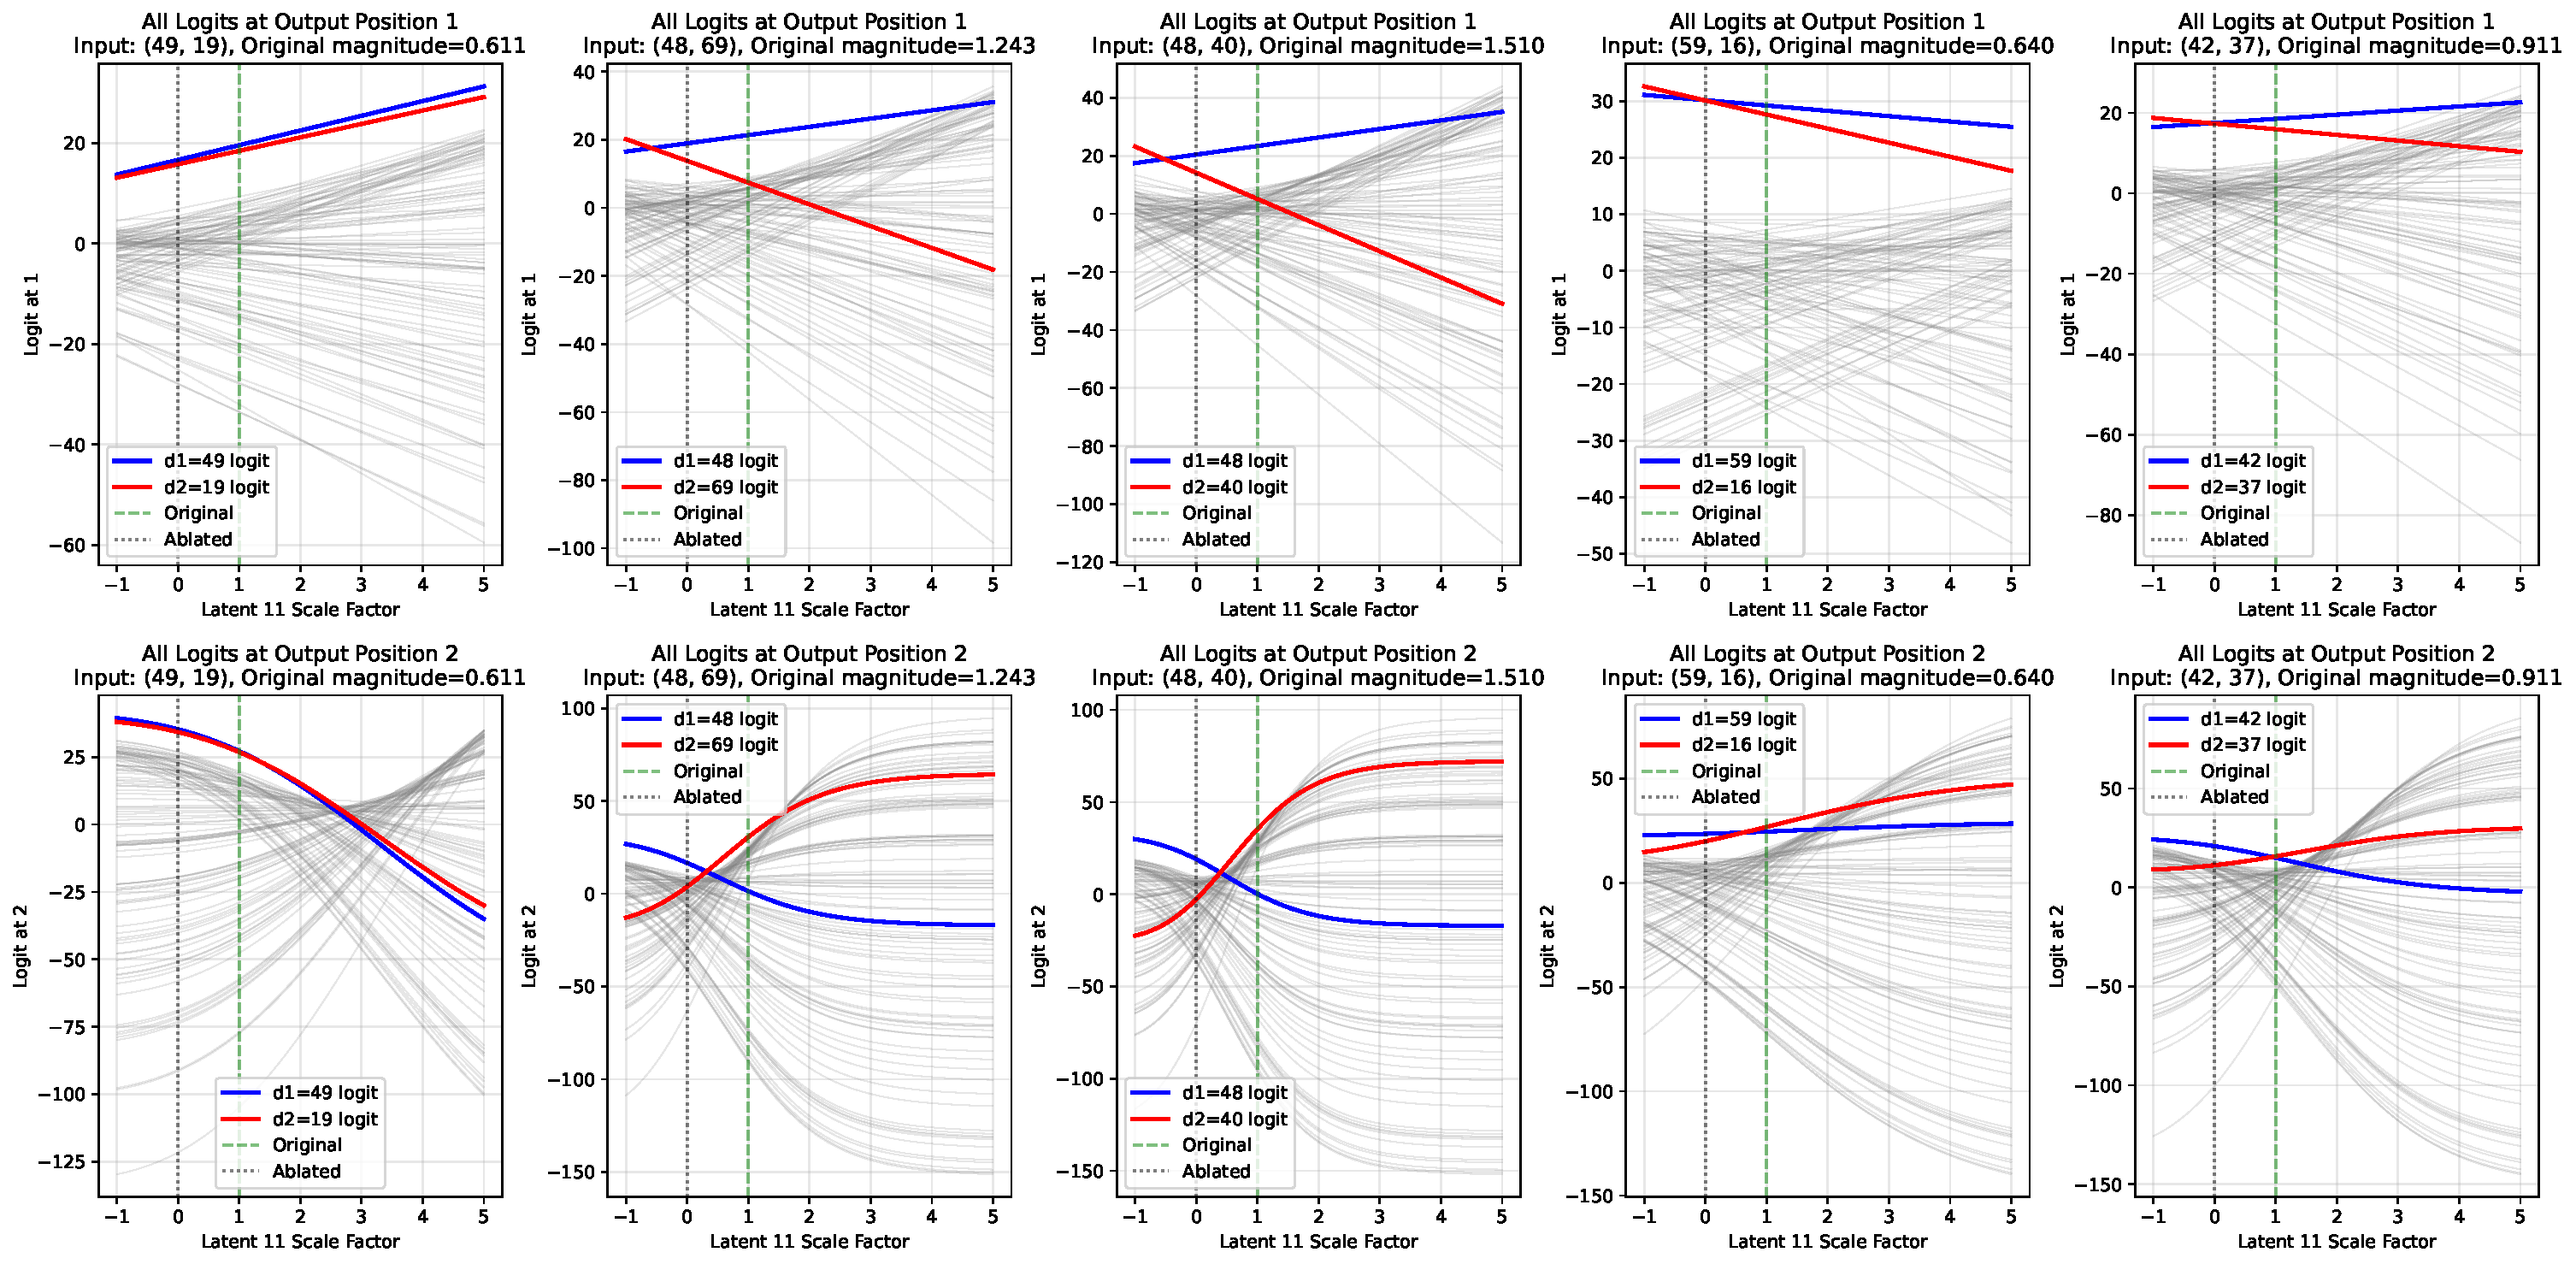
\includegraphics[width=\linewidth]{figures/steering_feat11_o1_negative_scale.pdf}
    \caption{
        For 9.2\% of inputs, latent 11 (in the BatchTopK SAE from Section \ref{s:method_rq2}) must be negatively scaled to swap the predicted symbol at one of the output positions.
    }
    \label{fig:steering_feat11_o1_negative_scale}
\end{figure*} 

\begin{figure*}[htbp]
    \centering
    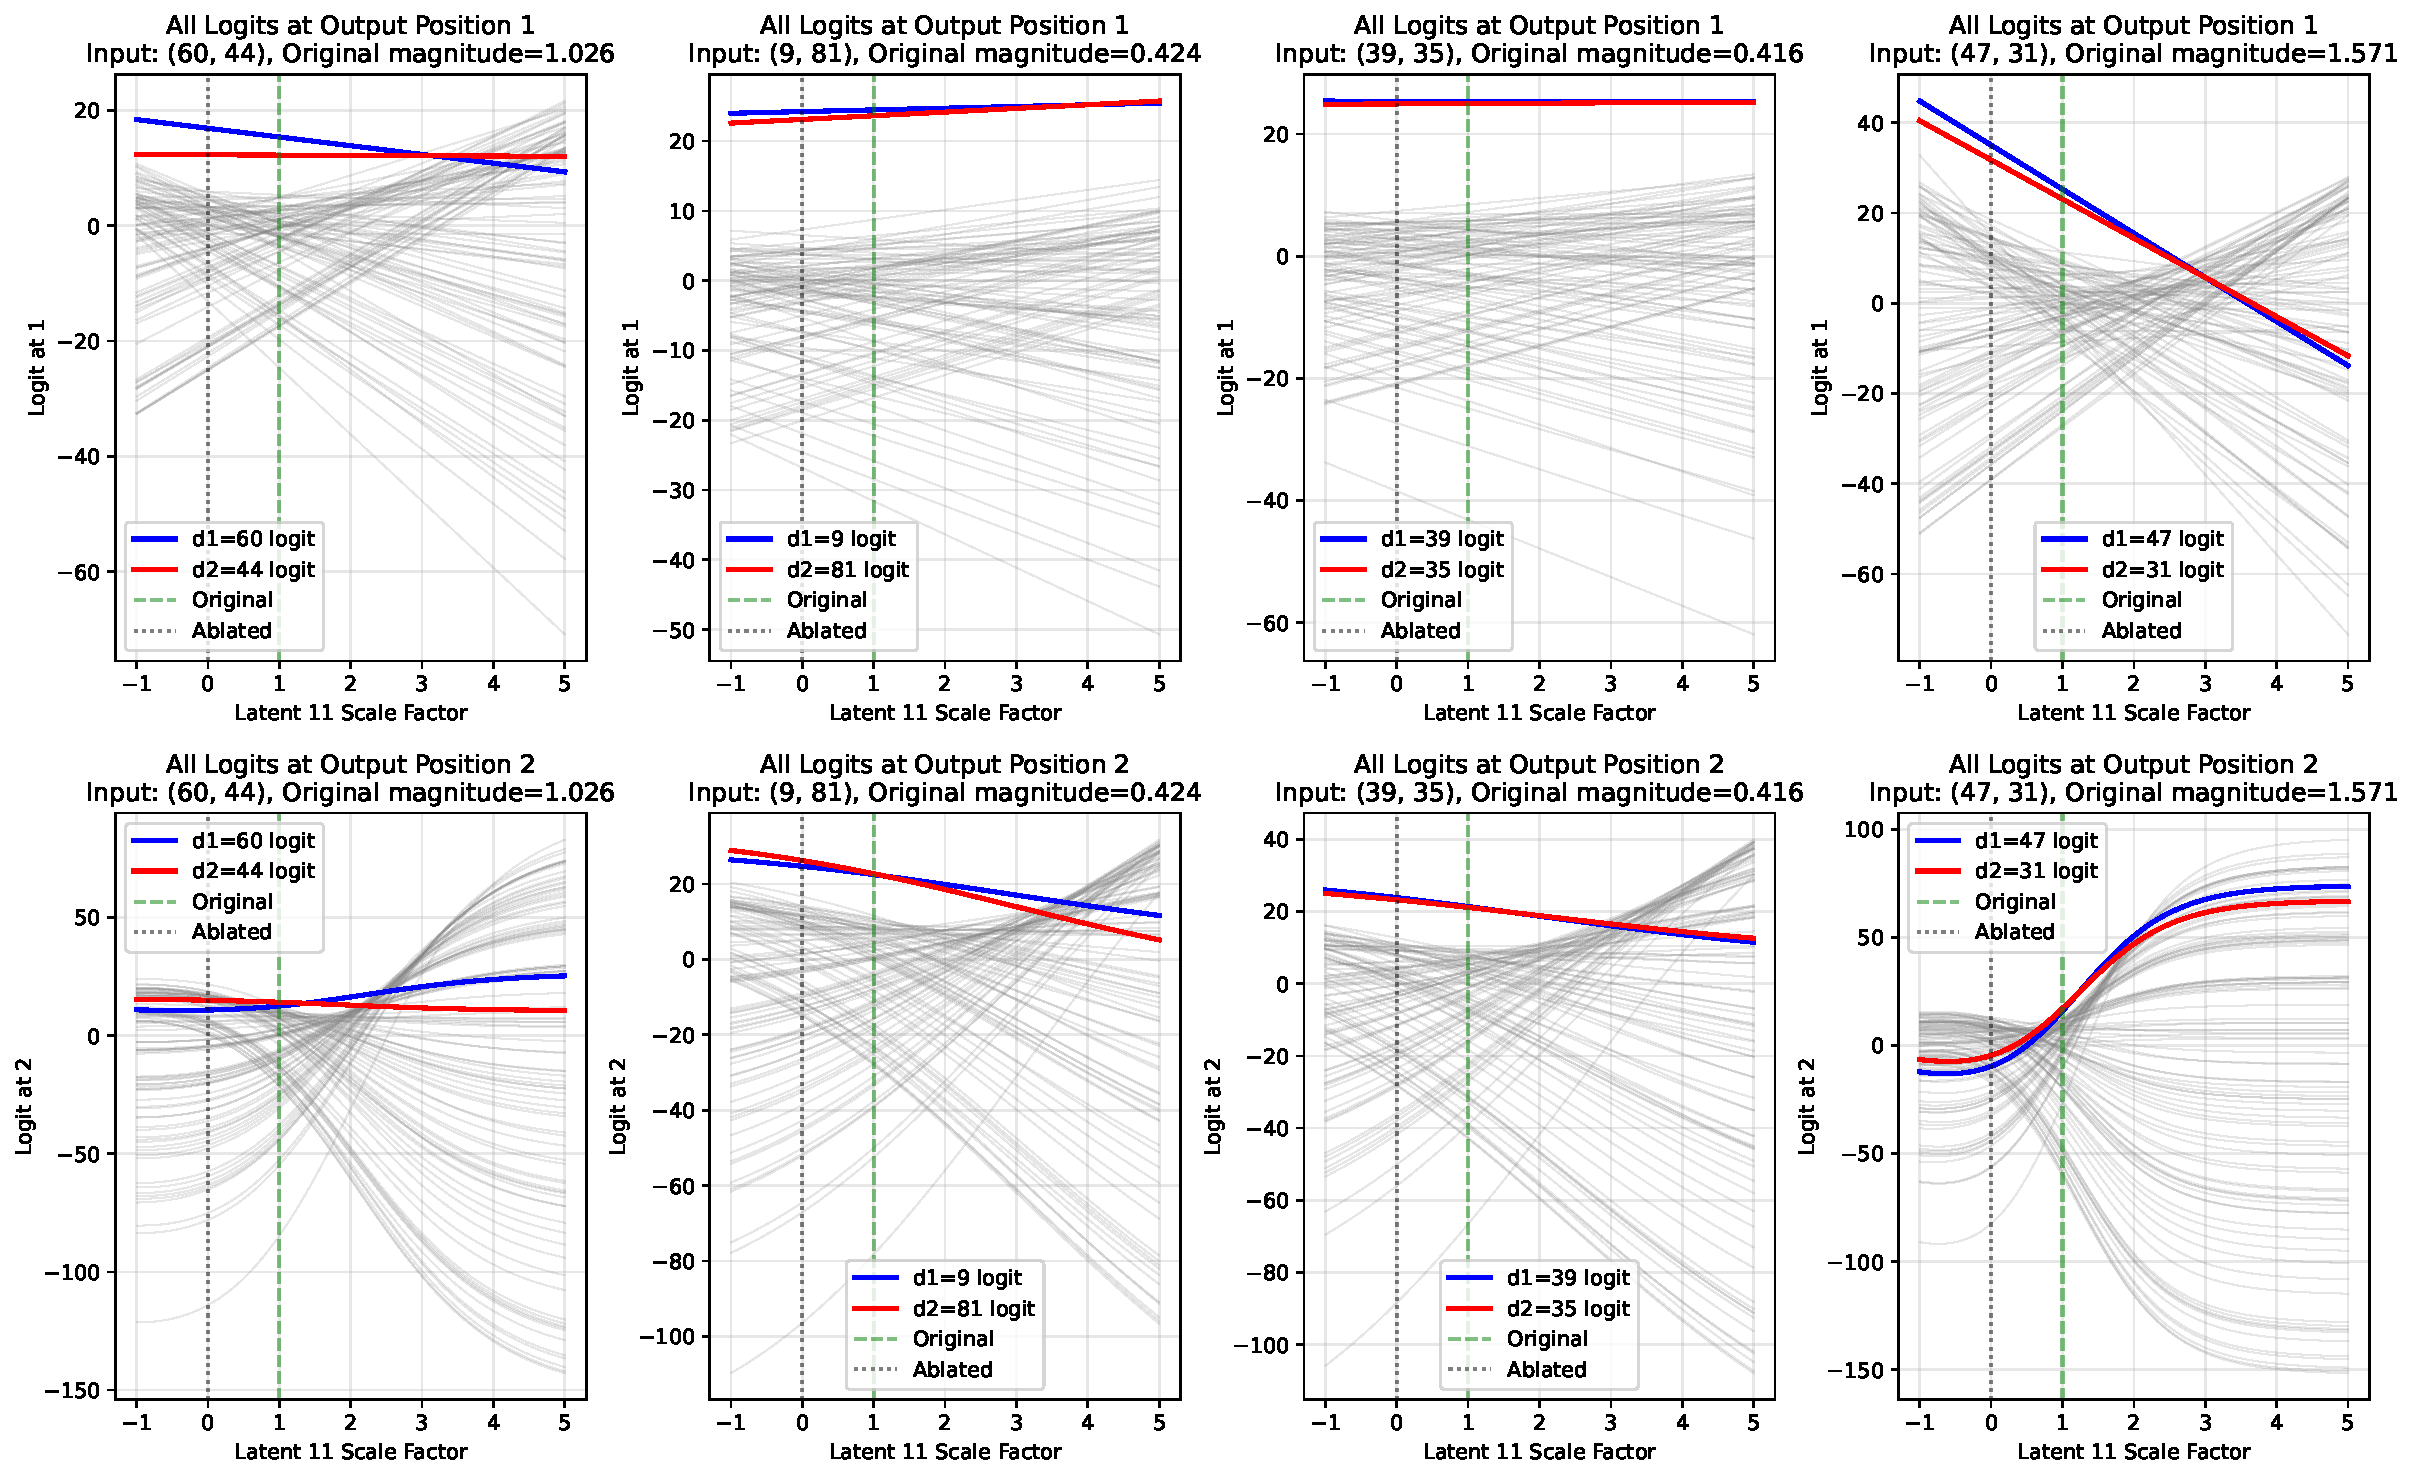
\includegraphics[width=\linewidth]{figures/steering_feat11_no_o2_crossover_in_bounds.pdf}
    \caption{
        For 2.3\% of inputs, it is possible to scale latent 11 (in the BatchTopK SAE from Section \ref{s:method_rq2}) to swap the symbol at each output position individually but not simultaneously.
    }
    \label{fig:steering_feat11_no_o2_crossover_in_bounds}
\end{figure*} 


\begin{figure*}[htbp]
    \centering
    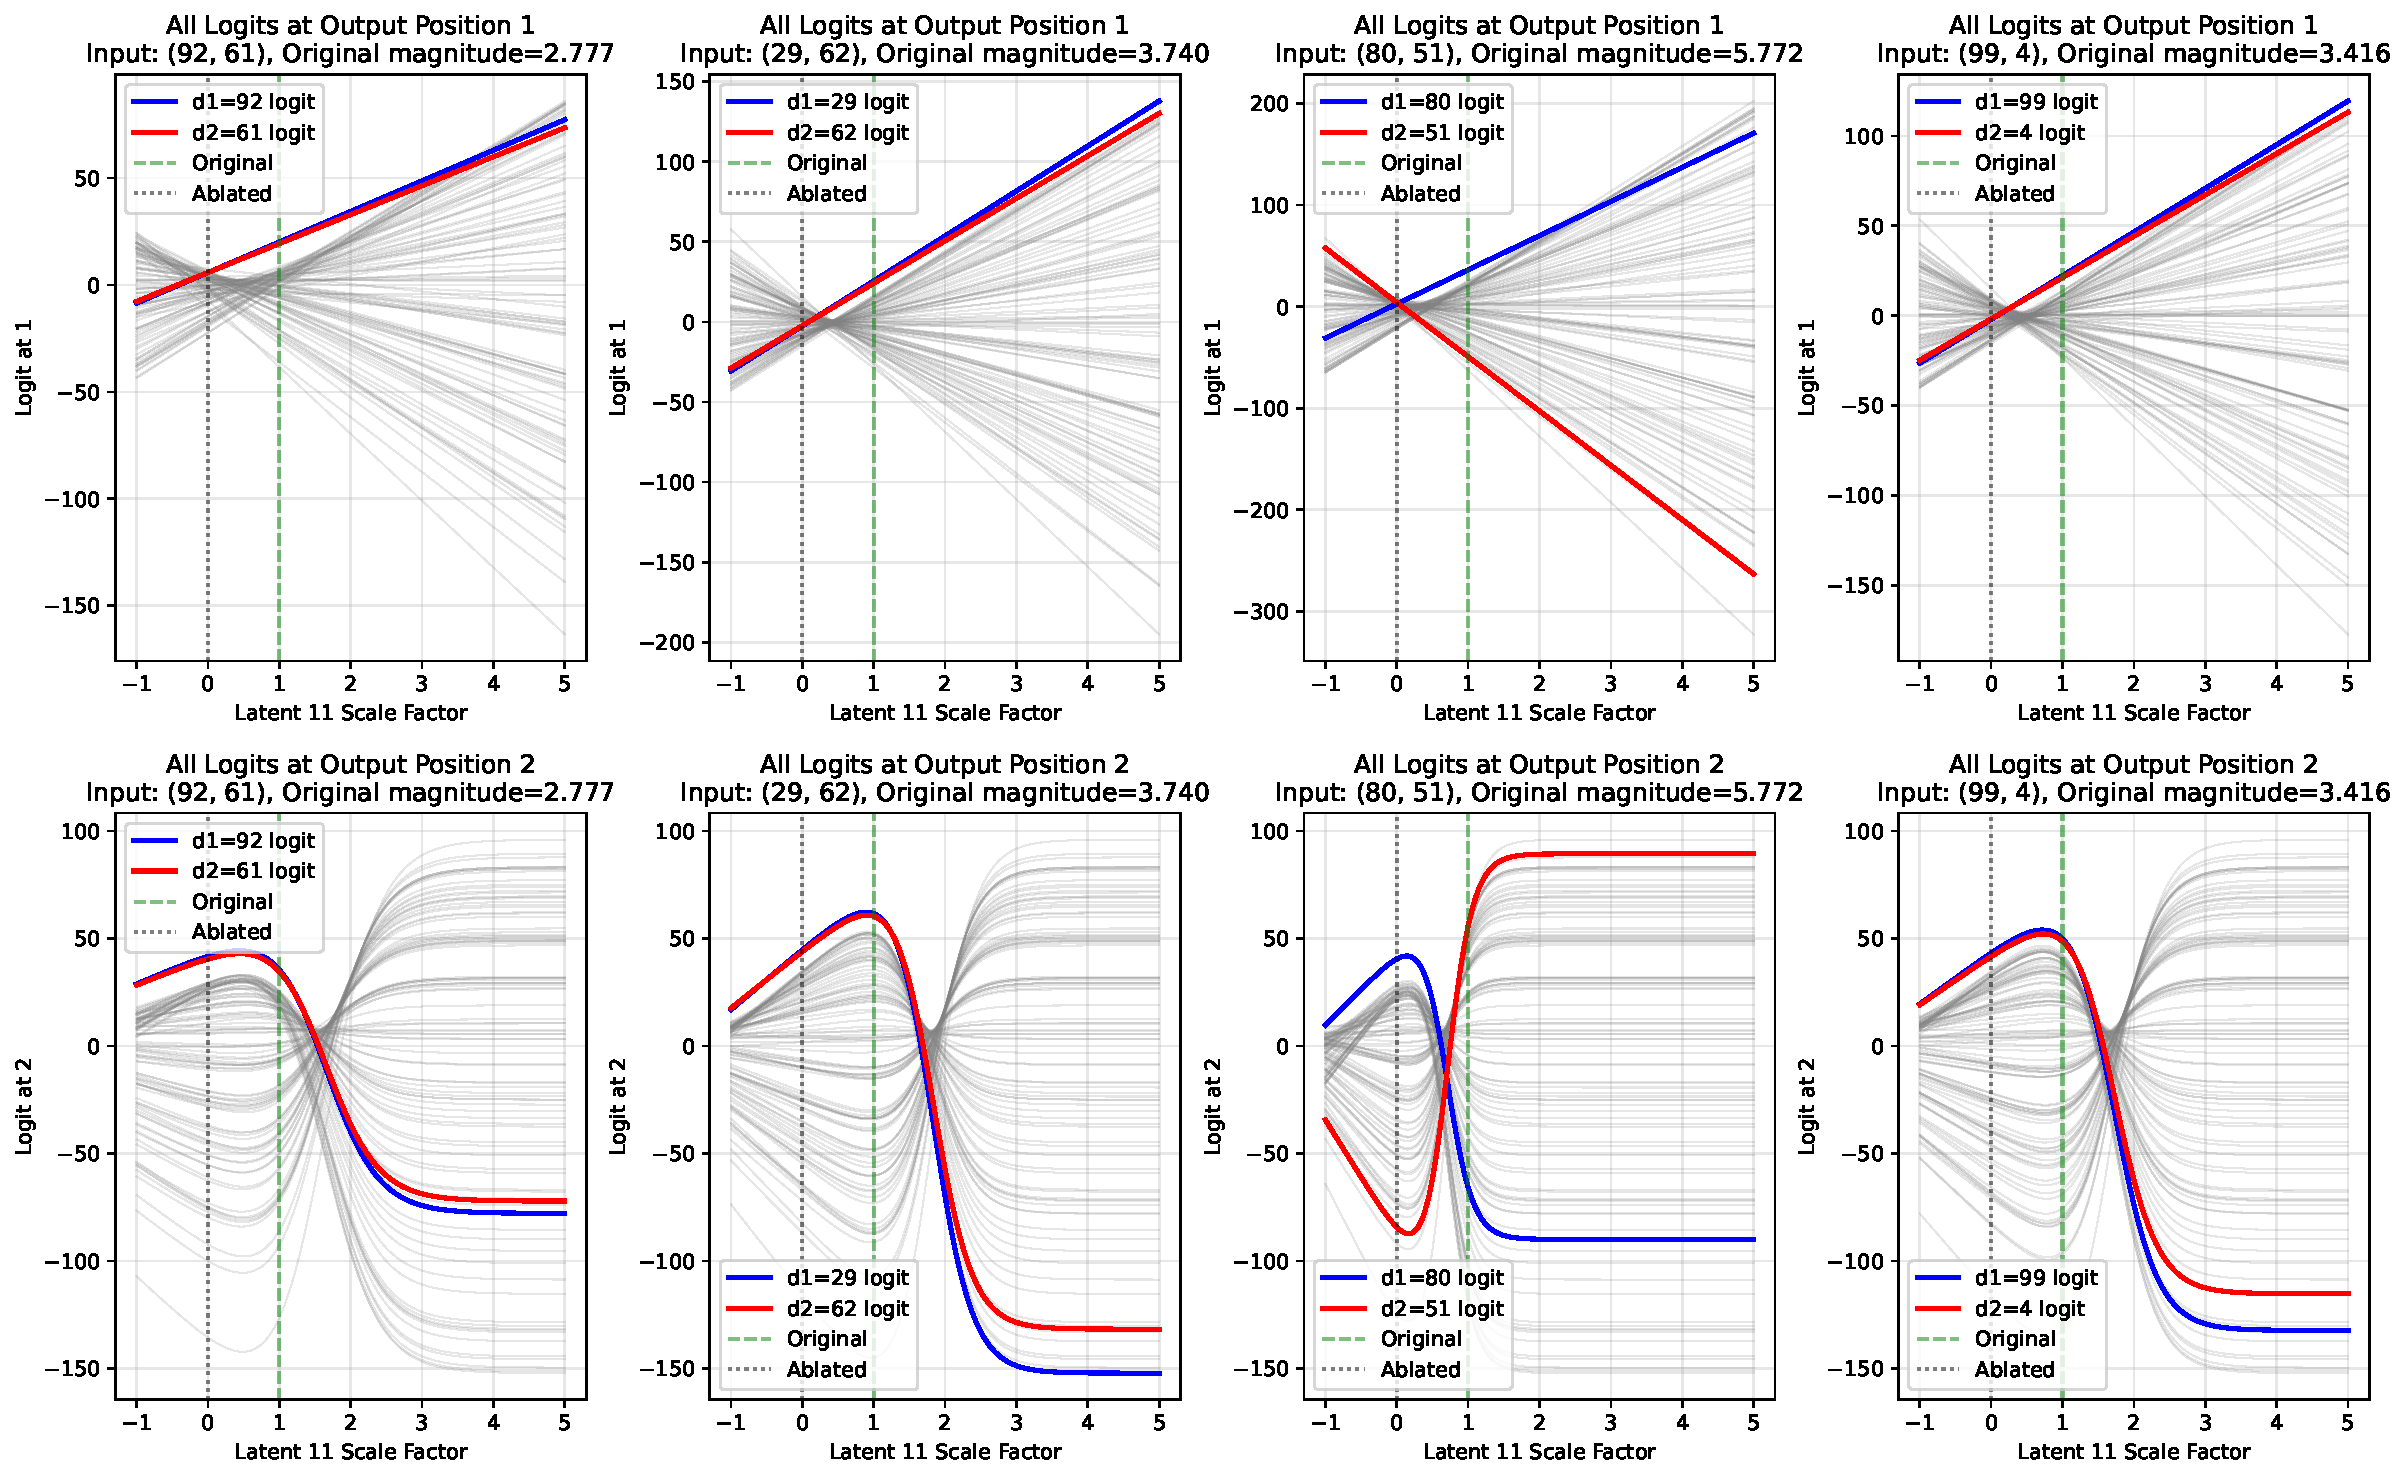
\includegraphics[width=\linewidth]{figures/steering_feat11_o1_never_predicts_d2.pdf}
    \caption{
        For 1.6\% of inputs, the logit for the symbol at $d_2$ is always dominant at $o_2$ in the observed latent scale range (in the BatchTopK SAE from Section \ref{s:method_rq2}), so there is no scale where the the symbol at $d_1$ is predicted instead.
    }
    \label{fig:steering_feat11_o1_never_predicts_d2}
\end{figure*} 

\begin{figure*}[htbp]
    \centering
    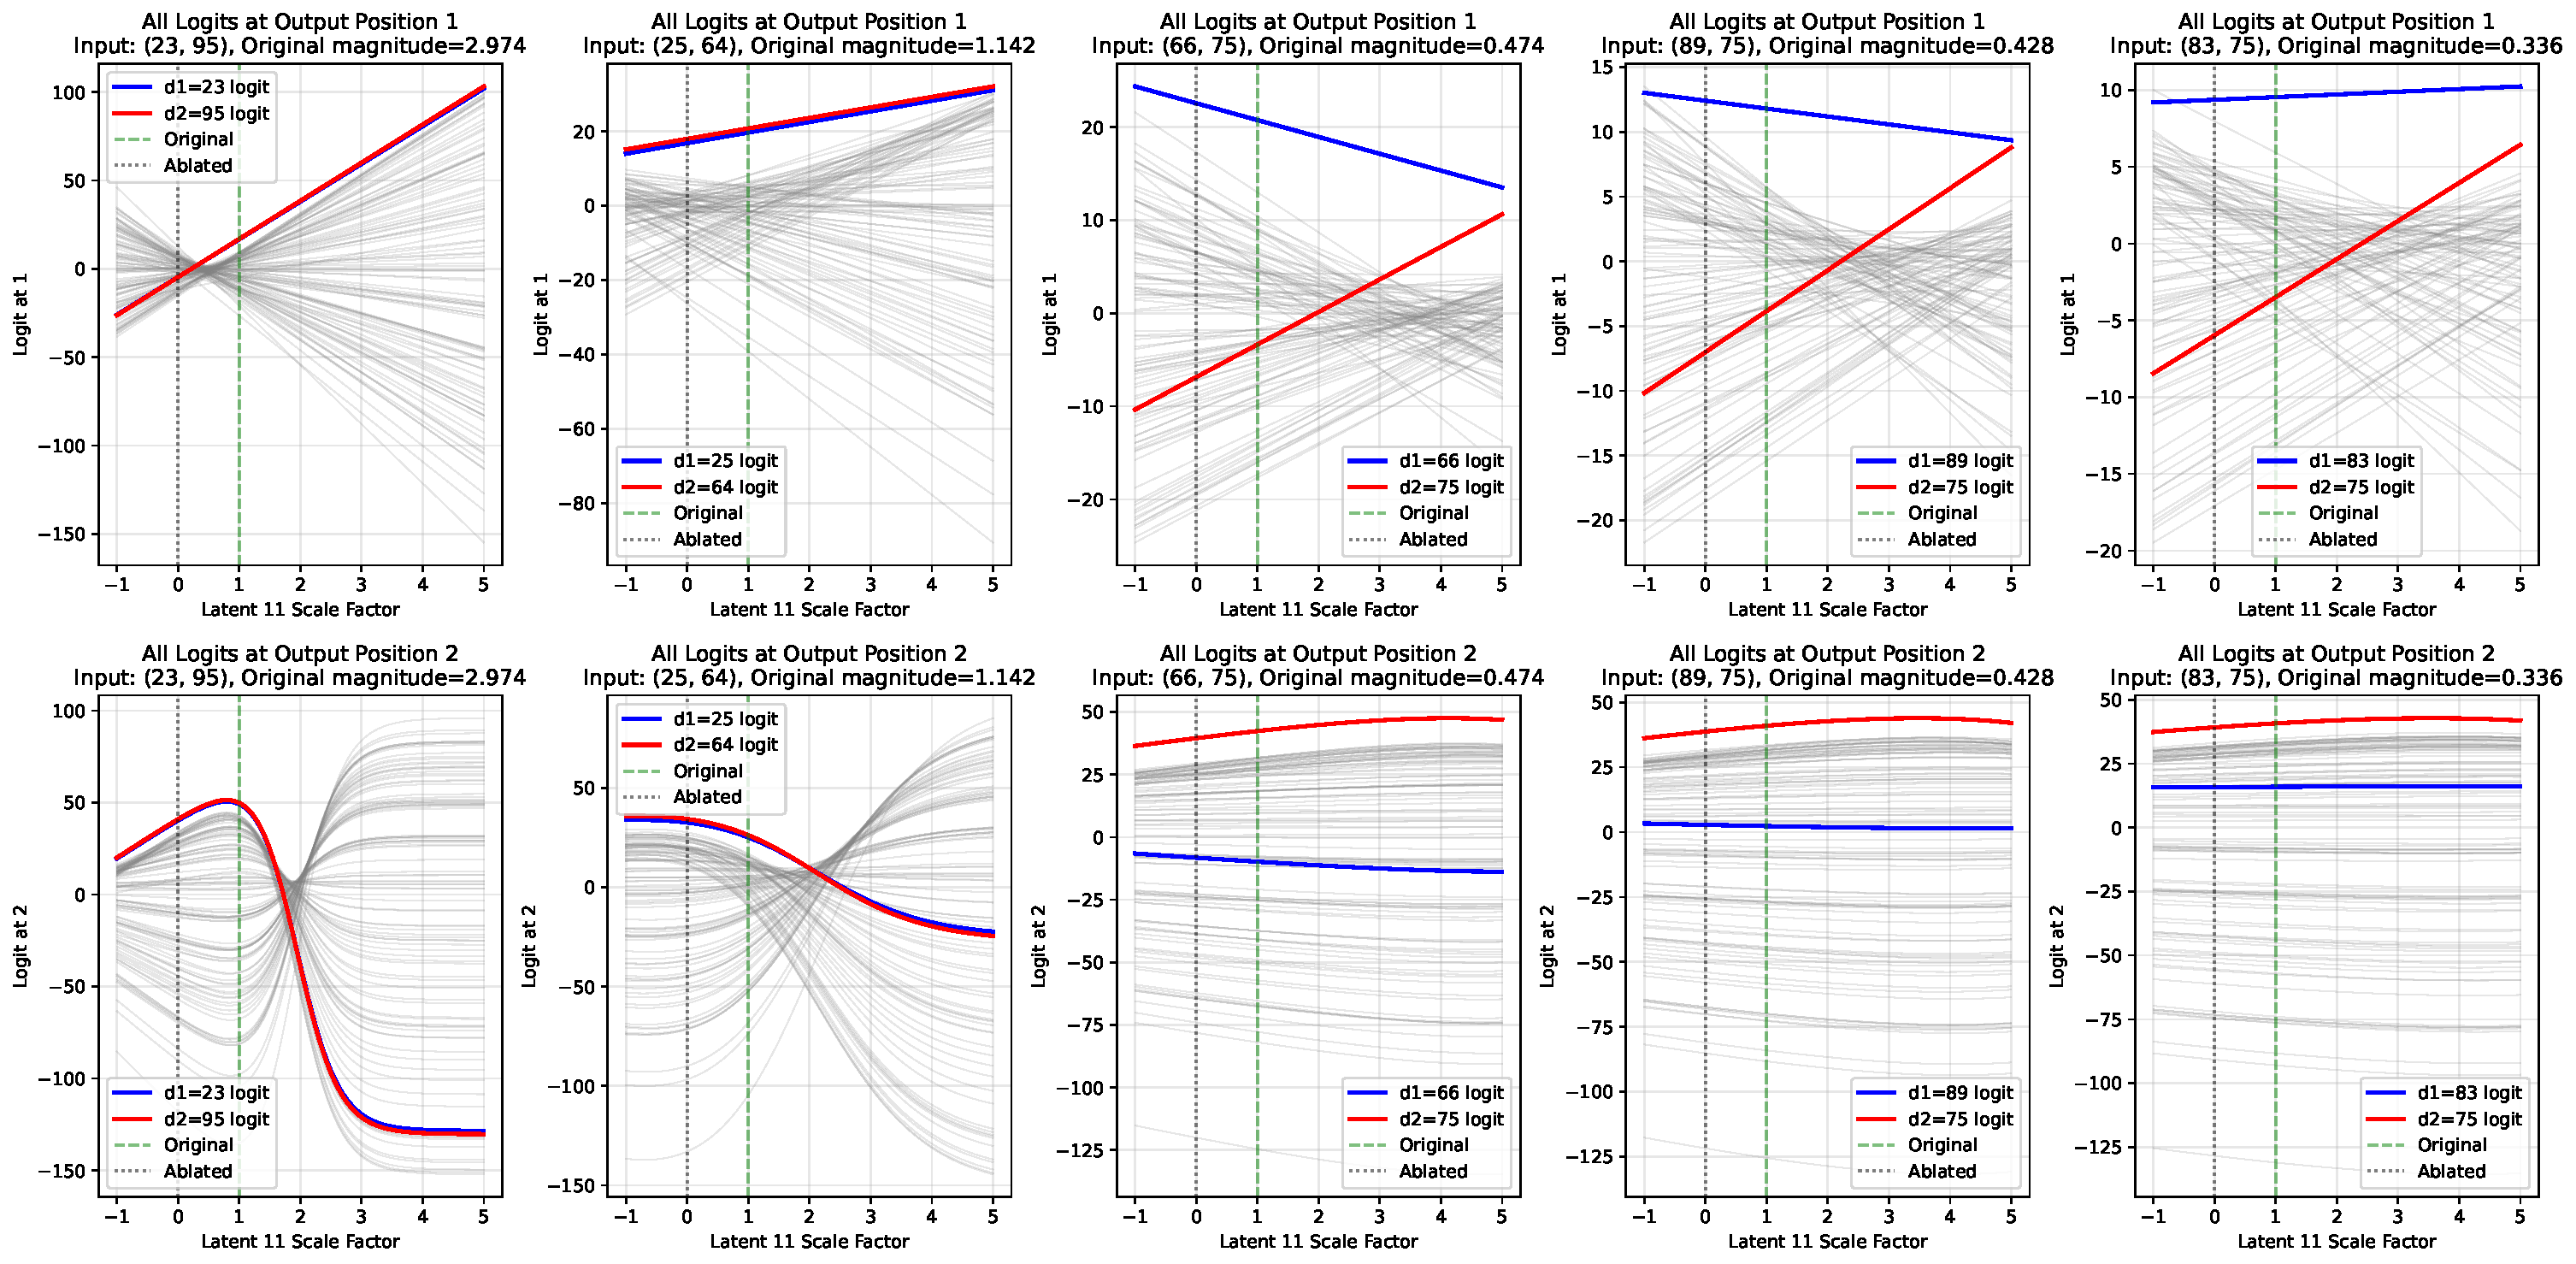
\includegraphics[width=\linewidth]{figures/steering_feat11_o2_never_predicts_d1.pdf}
    \caption{
        For 0.2\% of inputs, the logit for the symbol at $d_1$ is always dominant at $o_1$ in the observed latent scale range (in the BatchTopK SAE from Section \ref{s:method_rq2}), so there is no scale where the the symbol at $d_2$ is predicted instead.
    }
    \label{fig:steering_feat11_o2_never_predicts_d1}
\end{figure*} 


\begin{figure*}[htbp]
    \centering
    \begin{minipage}[t]{0.3\linewidth}
        \centering
        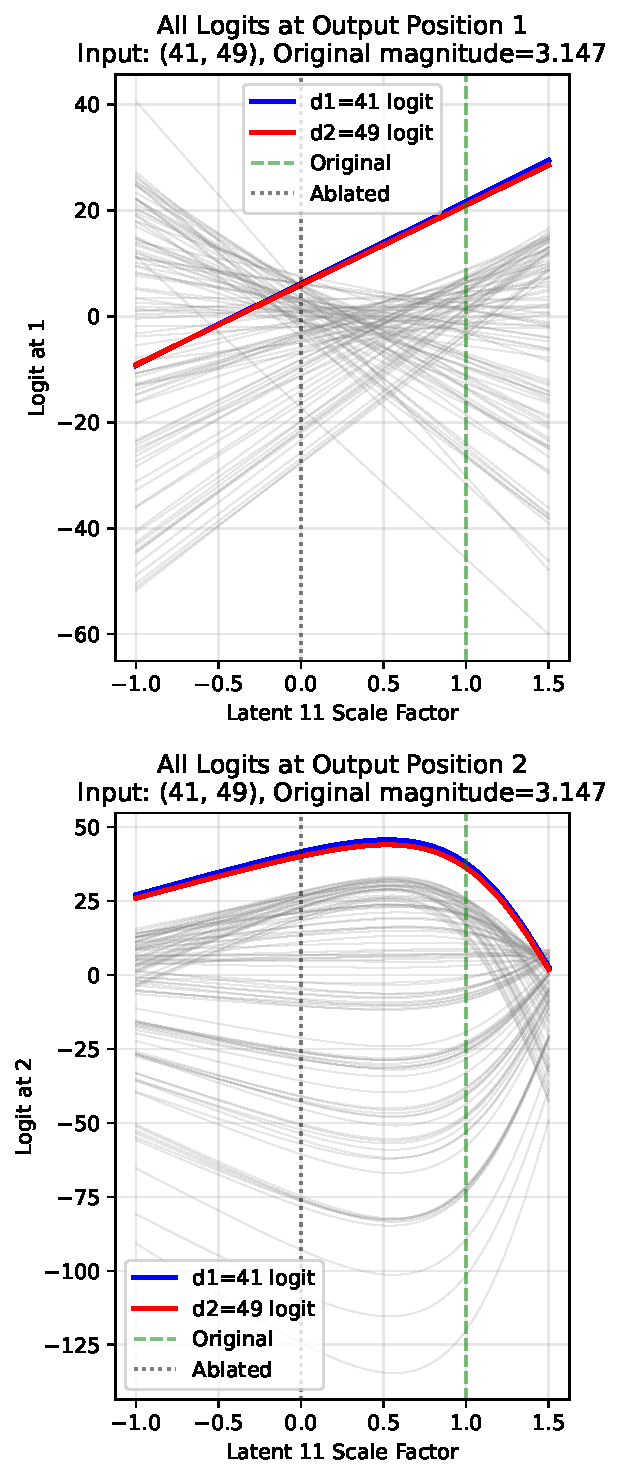
\includegraphics[width=\linewidth]{figures/41_49_a.pdf}
        \caption{
            In the BatchTopK SAE from Section \ref{s:method_rq2}, latent 11 cannot be scaled to swap input bigram $(41,49)$ because the logit for $49$ is never argmax in position $o_1$, as shown by the top plot.
        }
        \label{fig:41_49_a}
    \end{minipage}
    \hfill
    \begin{minipage}[t]{0.3\linewidth}
        \centering
        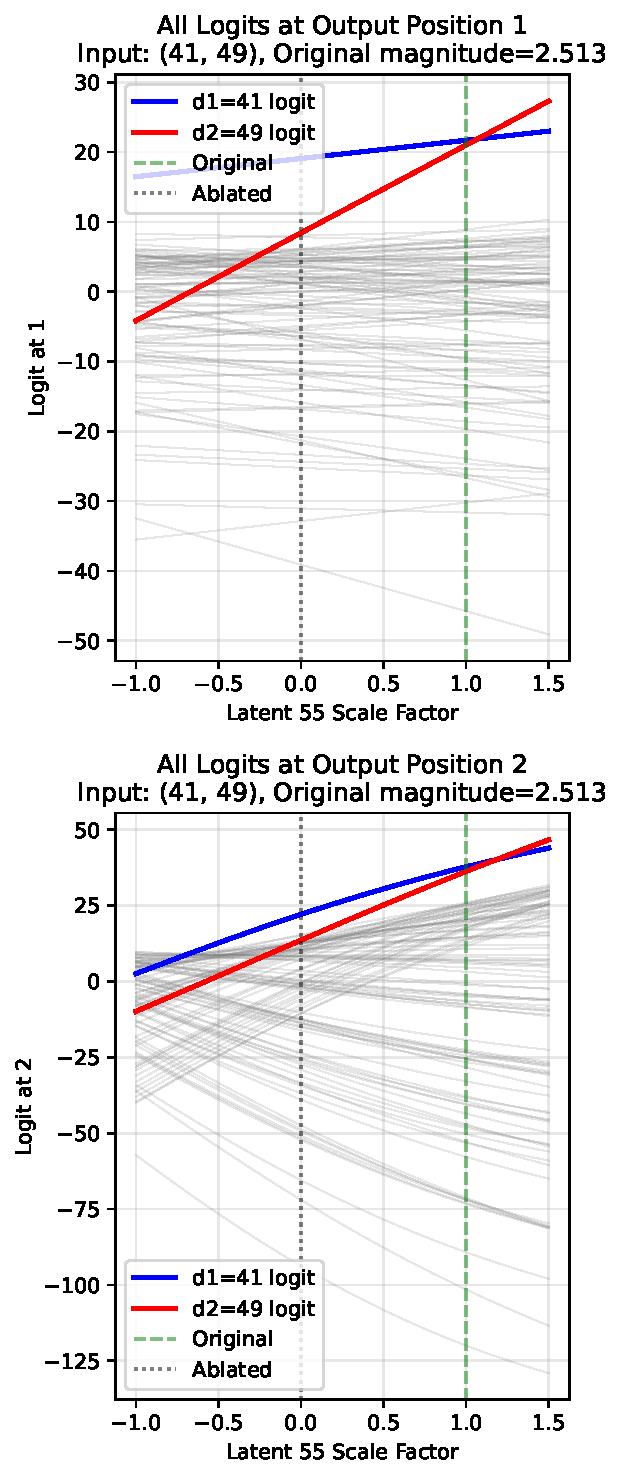
\includegraphics[width=\linewidth]{figures/41_49_b.pdf}
        \caption{
            However, in the same SAE, latent 55 co-activates with latent 11 for input $(41,49)$ and can be scaled by factor $p \in [1.07, 1.18]$ to cause the model to output $(49,41)$ instead.
        }
        \label{fig:41_49_b}
    \end{minipage}
    \hfill
    \begin{minipage}[t]{0.3\linewidth}
        \centering
        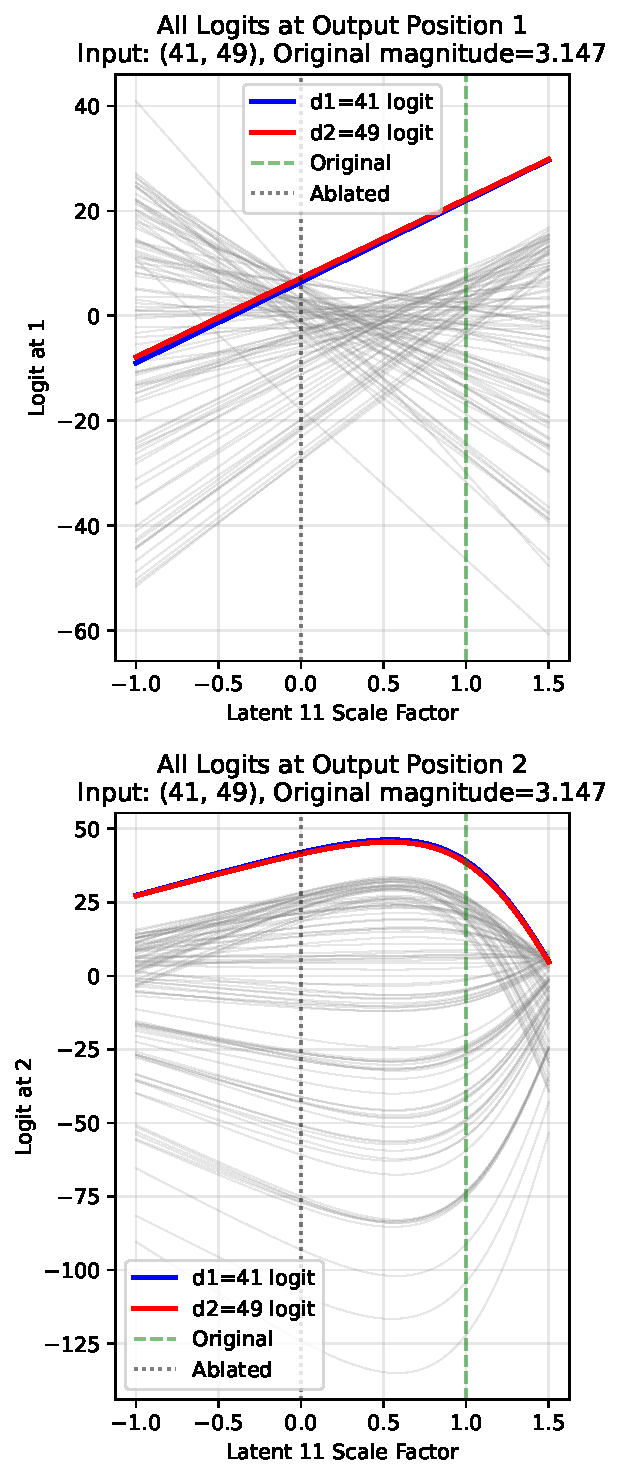
\includegraphics[width=\linewidth]{figures/41_49_c.pdf}
        \caption{
            Moreover, in the same SAE, if latent 55's activation magnitude is scaled by a factor of 1.1, then we can now scale latent 11 by factor $p \in [0.03, 1.45]$ to swap the outputs, which was not possible without scaling latent 55. This suggests that some graded activation demonstrations are only possible when multiple active latents are scaled simultaneously.
        }
        \label{fig:41_49_c}
    \end{minipage}
    % \caption{
    %     TODO overall
    % }
\end{figure*}